% !TEX encoding = UTF-8 Unicode 
% !TEX root = praca.tex

\chapter{Implementation of sample applications}

In this chapter, the development of the sample applications is presented. The implementation is based on the research scenarios defined in chapter \ref{chap:research_scenarios}.

\section{Research scenario 1: List scrolling and filtering}

\begin{figure}
    \begin{minipage}{.47\textwidth}
      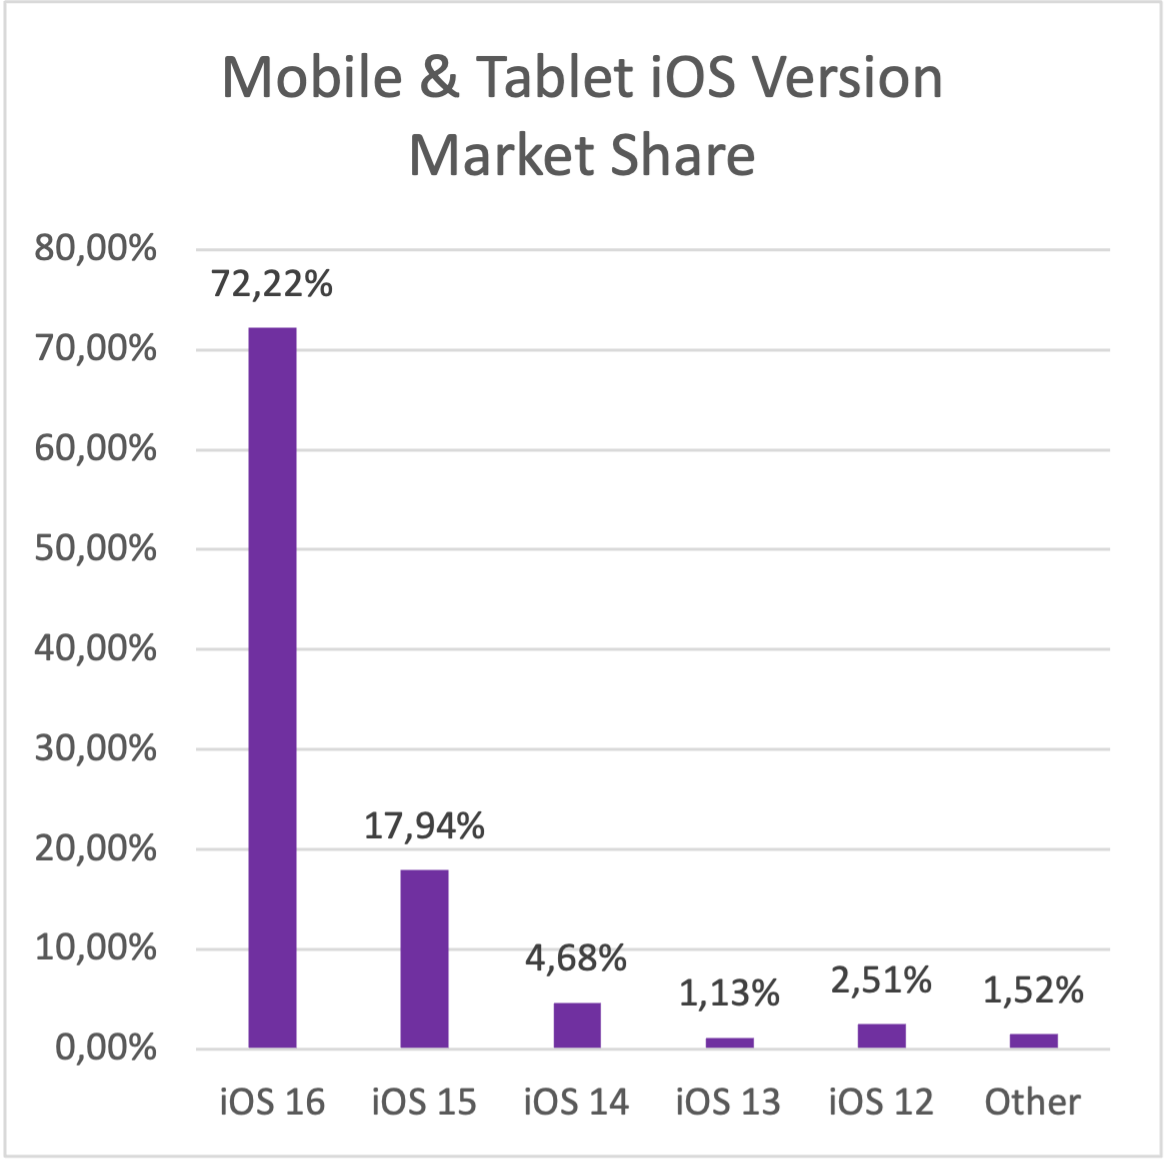
\includegraphics[width=.5\textwidth]{img/ios_ver_market_share}
      \caption{App 1: Kotlin (Source: Own work)}
      \label{fig:app1_kotlin}
    \end{minipage}
    \hfill
    \begin{minipage}{.47\textwidth}
      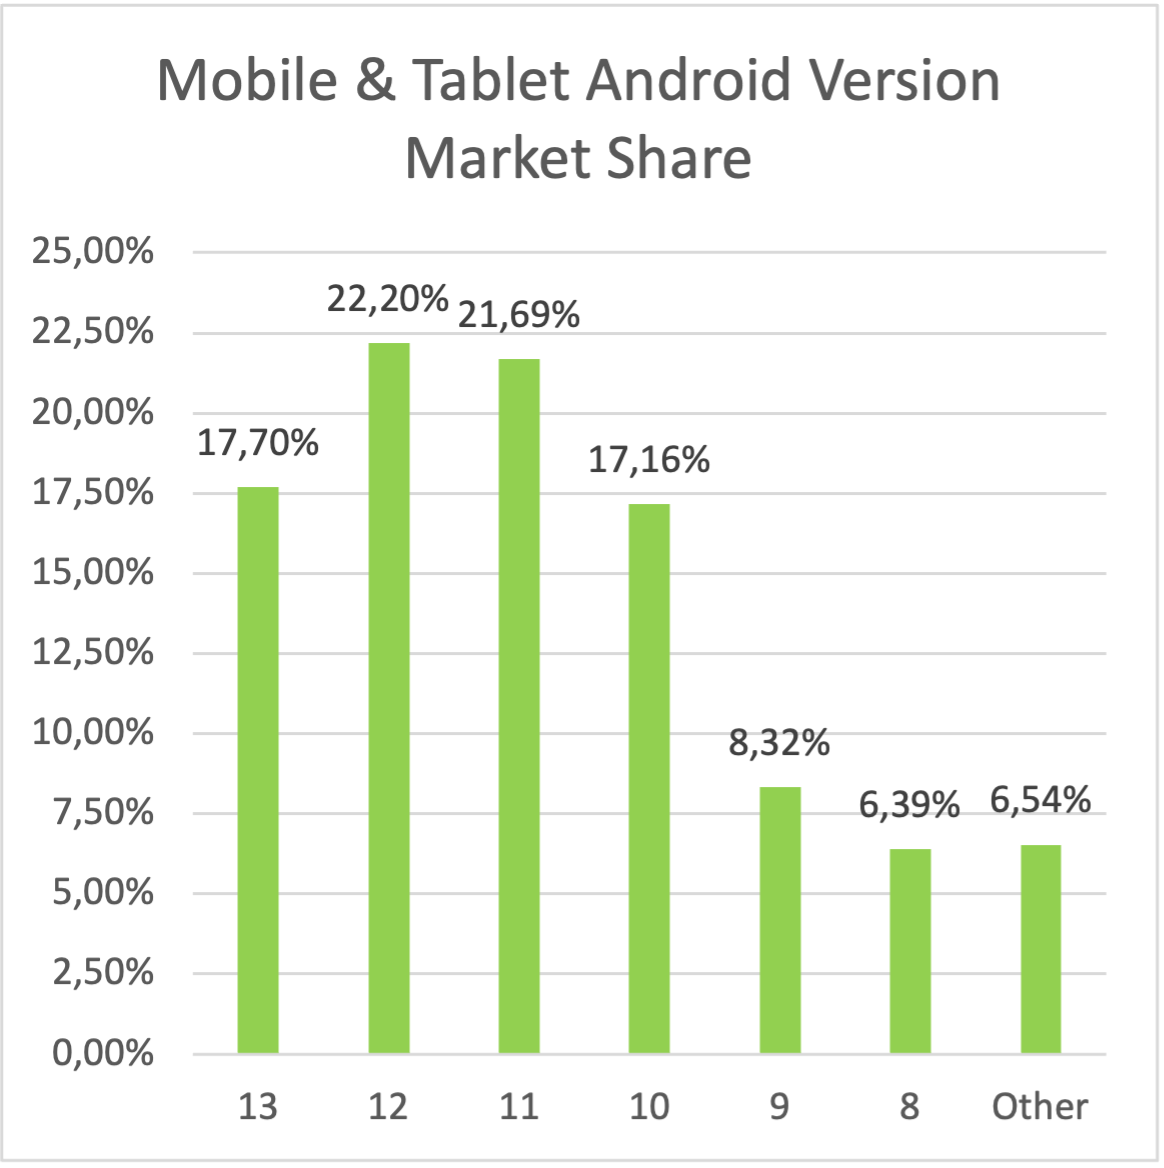
\includegraphics[width=\textwidth]{img/android_ver_market_share}
      \caption{App 1: Swift (Source: Own work)}
      \label{fig:app1_swift}
    \end{minipage}
\end{figure}

\begin{figure}
    \begin{minipage}{.47\textwidth}
        \centering
        \includegraphics[width=.6\textwidth]{img/app1_flutter}
        \caption{App 1: Flutter (Source: Own work)}
        \label{fig:app1_flutter}
      \end{minipage}
      \hfill
      \begin{minipage}{.47\textwidth}
        \centering
        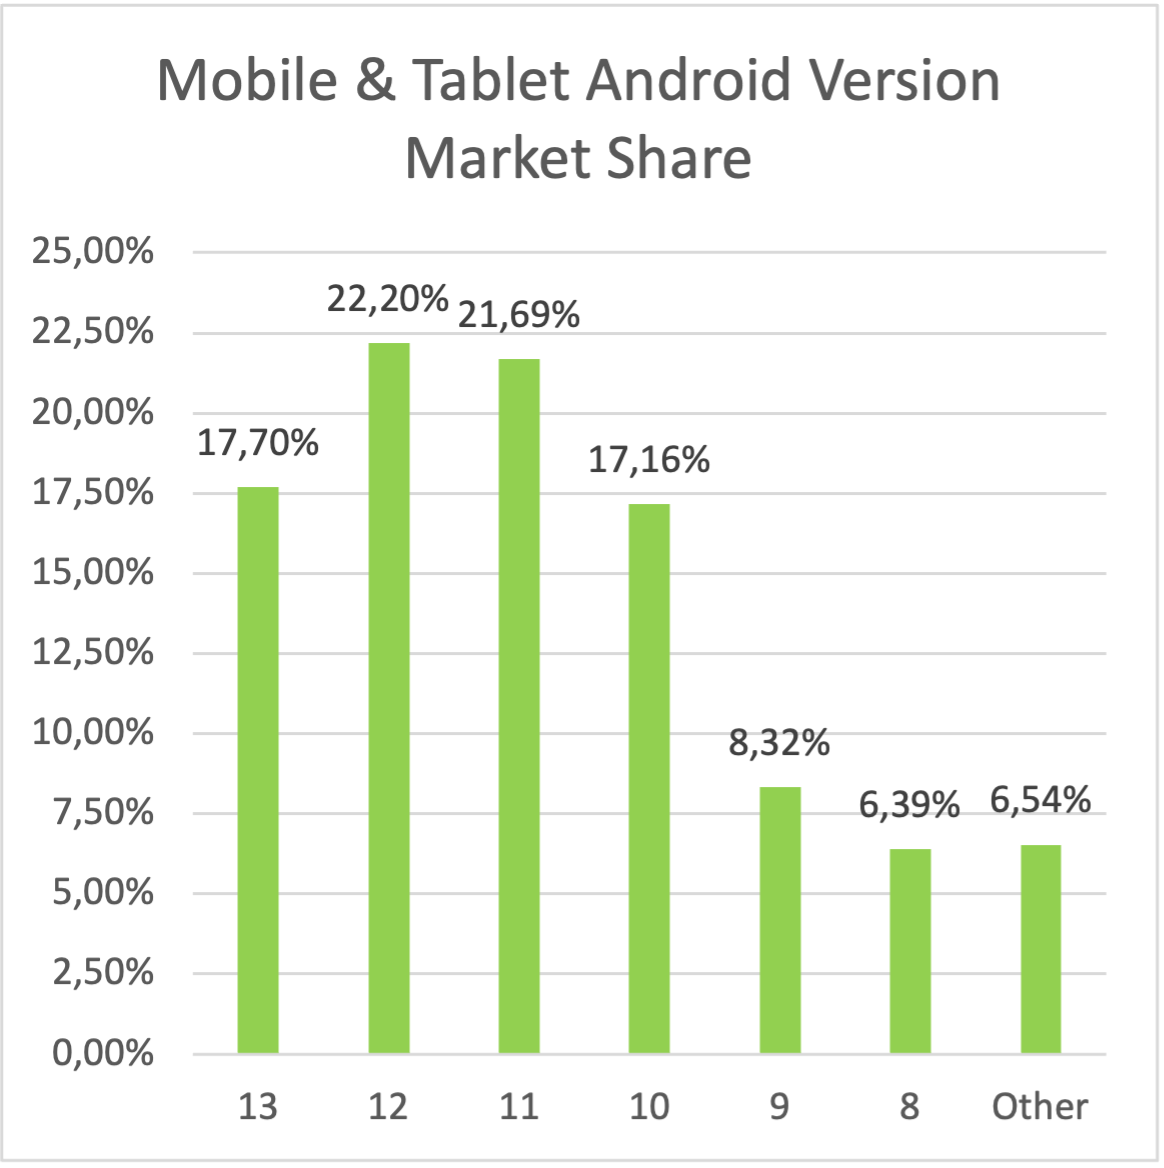
\includegraphics[width=.6\textwidth]{img/android_ver_market_share}
        \caption{App 1: React Native (Source: Own work)}
        \label{fig:app1_react_native}
      \end{minipage}
\end{figure}

\section{Research scenario 2: Animations}

\section{Research scenario 3: File I/O}

\section{Research scenario 4: Common UI elements}
